\chapter{Concepts}



While \parencite[p. 66]{Botjes2020} defined optionality as part of diversity the definitions are slightly different. In the case of this research it is applicable to use both the concepts.
\begin{remark}
Needs some references to taleb and others to do so in the case of my research.
\end{remark}

\section{Questions for Interviews}
\label{sec:questionsforinterviews}
The questions for the interviews are limited by the constraint of time of an interview. Because of this time constraint I limited the number of questions to five. However the five questions do cover the attributes of \gls{antifragile} and the concept of \gls{ea}.



Architects use an \gls{archframework} for describing \acrshort{ea}. Most of the frameworks use a layered approach for specific viewpoints on a system. The most used layers are business, information, applications, and technology. \textcite[p. 189]{Ylimaeki2005} suggests that \acrshort{ea} is an approach for controlling the complexity and constant changes in the business environment of an organisation, enabling alignment between the business vision, business requirements and information systems.


Most people answer that the opposite of \gls{fragile} is \gls{robust}, \gls{resilient}, solid, or something of the sort. However, the \gls{resilient}, \gls{robust} (and company) are items that neither break nor improve, so you would not need to write anything on them — have you ever seen a package with \gls{robust} in thick green letters stamped on it? Logically, the exact opposite of a \gls{fragile} parcel would be a package on which one has written; please mishandle or please handle carelessly. Its contents would not just be unbreakable but would benefit from shocks and a wide array of trauma \parencite{Taleb2012}. \textcite[p. 32]{Botjes2020} mentions that almost all if not all papers on antifragility and resilience use the term stressor for an event from outside the system that causes stress.



\textcite[p. 32]{Botjes2020} mentions that almost all if not all papers on antifragility and resilience use the term stressor for an event from outside the system that causes stress. 

\begin{figure}[h!]
	\centering
	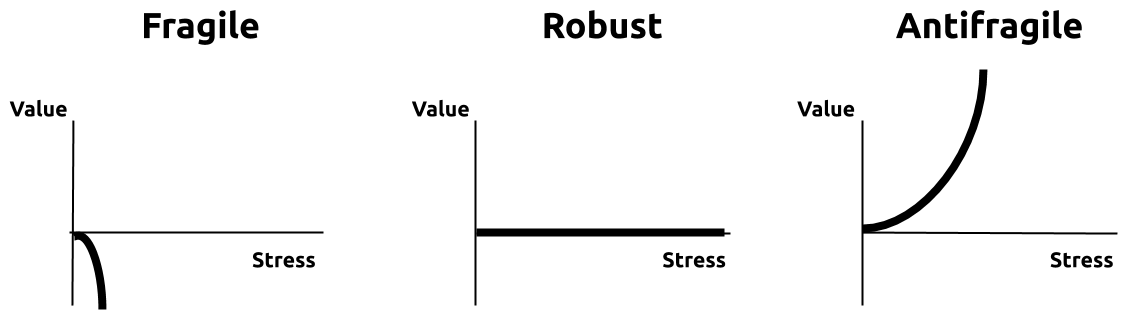
\includegraphics[width=0.7\linewidth]{images/eaal-triad}
	\caption[EAAL Triad]{\acrfull{eaal} Triad \parencite{Botjes2020}}
	\label{fig:eaal-triad}
\end{figure}


\begin{remark}
	Can the same principles on Concerns and Cohesion be used to cope with stressors or black swans (for the stable part of Seneca Barbell)? What is the relation of Modularity with the Variation (and that other one) of Antifragile.
\end{remark}

\section{af parts}


''Define antifragility as a property of a system'' \parencite{Jaaron2014}. \textcite{Kastner2017} created a framework for designing an antifragile organisation: Antifragile Organisation Design Framework. The framework consists out of 4 main principles:
\begin{itemize}
	\item{\textbf{Self Organisation.} Decentralisation can be seen as a strategy for organisational survival \parencite{Brafman2007}.}
	\item{\textbf{Ownership.} Result based and 'Skinin the game'.}
	\item{\textbf{Diversity of cells and organisational learning.}}
	\item{\textbf{DNA - Shared purpose, values and culture.}}
\end{itemize}

Decentralised Systems, using self organising capabilities might not only survive disruptions but could even prosper \parencite{Brafman2007}.The only real difference with Complex Adaptive System and antifragile of \textcite{Taleb2012} is that with antifragile stressors, disruptions, errors, volatility, randomness, chaos and uncertainty are seen as 'desired events' in order to strengten and evolve the system \parencite{Jaaron2014}.\\

To build an antifragile system there are three main concepts to follow \parencite{Russo2017}.
\begin{itemize}
	\item{Since antifragile means to benefit more than to loose (positive asymmetry), the first step is to reduce possible losses.}
	\item{The second step is to avoid disastrous scenarios by hedging correctly risks.}
	\item{The last step is to embed adaptive fault tolerance.}
\end{itemize}

Some authors propose also a fault injection approach, to increase the numbers of errors to enhance the
learning capabilities \parencite{Russo2017}.
\begin{remark}
	This is the method of Antidotum Mithridatium \parencite{Taleb2012}.
\end{remark}

\begin{remark}
	for systems resilience Kastner loc 327 contains three references that have to be used for reference on robustness.
\end{remark}
Three key sytems properties contribute to its resilience \parencite[p. 9]{MartinBreen2011}:
\begin{itemize}
	\item{Diversity and Redundancy}
	\item{Modular Networks}
	\item{Responsive, regulatory feedbacks.}
\end{itemize}
For resilience one not only needs to answer the questions ''Resilience of what?'' and ''Resilience to what?'', but also ''Resilience for whom?'' \parencite[p. 21]{Lebel2006}. One can apply basic critical systems design principles to spot ways to maintain any system's function in the event of a crisis \parencite[p. 10]{MartinBreen2011}:
\begin{itemize}
	\item{Maintain a diversity of mechanisms to provide identical functions.}
	\item{Make sure networks (social or otherwise) are modular enough so damange or ''infection'' of one portion does not immediately propogate to all others.}
	\item{Maintain or establish feedbacks to, in the simplest case, establish fail0safe mechanisms in case of malfunction.}
\end{itemize}
One can maximize efficiency over all of these variables; however, such optimisation assumes full working knowledge of the system.
\begin{remark}
	Enterprise architecture can be used to give this full working knowledge of the system.
\end{remark}

The term resilience (including all three examined concepts) focuses on the avoidance of harmfull stressors and failure; and uncertainty and volatility. Moreover, these are even constructed to reduce vulnerability as much as possible \parencite{MartinBreen2011}.
\begin{remark}
	add extra references from Kastner to this cite.
\end{remark}

\subsection{EAAL Model}
\label{sub:eaal}

\textcite{Botjes2020} has conducted literature research for his master project. This literature research was used to define the defintions of \gls{antifragility} and to define attributes relevant to \gls{antifragility}. The outcome of this research is the \acrfull{eaal} model. The outcome of the research of \textcite{Botjes2020} also stated that the attributes of \gls{antifragility} are additional to those of \gls{resiliency}. Therefor \acrshort{eaal} model contains an overview on not only the attributes of \gls{antifragility}.

\begin{figure}[H]
	\centering
	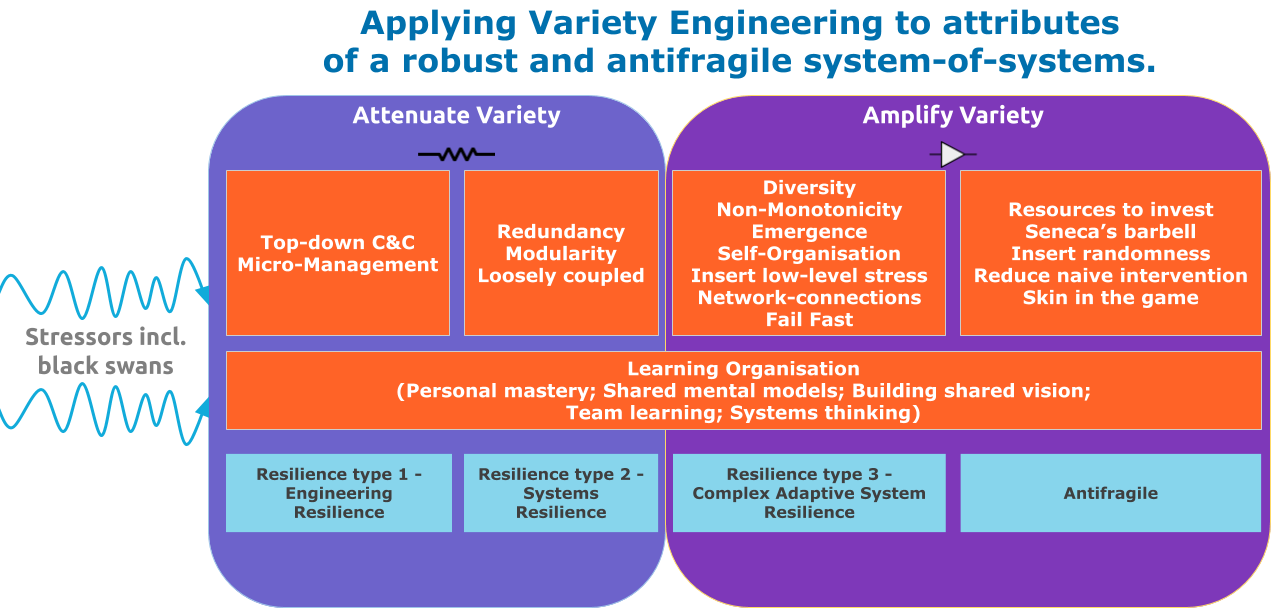
\includegraphics[width=0.7\linewidth]{images/eaal}
	\caption[EAAL]{EAAL \parencite{Botjes2020}}
	\label{fig:eaal}
\end{figure}

The \acrshort{eaal} model of \parencite{Botjes2020} uses Variety Engineering \needsref as his base. The variety engineering consists out of two different varieties. The Attenuate Variety, and the Amplified Variety.

\begin{itemize}
	\item{\textbf{Attenuate Variety.}}
	\item{\textbf{Amplified Variety.}}
\end{itemize}

The more amplified variety a \acrshort{sos} has the more antifragile the \acrshort{sos} is \needsref.

\begin{remark}
	Need more information to be eleborated on this. The information should be from the source of Edzo.
	
	Edzo his paper contains references to ashley and beer about these kinds of variety!
	
\end{remark}

The research of \textcite{Botjes2020} is recent and contains a good overview of needed attributes for a system-of-systems to become more \gls{antifragile}.

\subsection{Antifragile Systems Design}
\label{sub:sfasd}




\begin{remark}
	
\end{remark}

Architects need to work with the business to describe the \acrshort{vuca} environment, translate the impacts on the
software decomposition, and even assist in business level mitigations \parencite[p. 886]{OReilly2019}.

\begin{remark}
	Is this only about software systems or also other systems like an organisation? Can it be generalised?
\end{remark}



The process of \acrshort{asd} constist out of four steps:
\begin{enumerate}
	\item{\textbf{\acrshort{vuca} Analysis.}}
	\item{\textbf{System Decomposition - Flow First Design.}}
	\item{\textbf{Design Testing.}}
	\item{\textbf{Modified \acrfull{fmea}}}
\end{enumerate}
\begin{remark}
	Needs some extra explanation per item
\end{remark}

Going forward, architects should consider the following actions \parencite[p. 889]{OReilly2019}:
\begin{itemize}
	\item{\textbf{Practice VUCA Analysis on the initiative's Business Model.}}
	\item{\textbf{Become an expert in system decomposition.}}
	\item{\textbf{Learn different methods for system decomposition.}}
	\item{\textbf{Learn to use modified \acrshort{fmea} to improve system designs.}}
\end{itemize}

\subsection{Residuality Theory}
\label{sub:sfresiduality}
Resilient systems are, by definition, able to survive disruption and eventually regain function. Beyond resilience is the
idea of antifragility – that systems actually learn from their exposure to stress and become stronger because of it \parencite{Taleb2012}\ \parencite[p. 876]{OReilly2020}. Residuality theory reveals a system as actually being made up of a stack of shadows which we cannot see without turning various lights on and off. We do this through a stressor analysis \parencite[p. 877]{OReilly2020}.

\begin{remark}
	The stack of shadows is related to ''the darkness principle'' \parencite[p. 78]{Richardson2004} from complexity science. This can be replaced with the original source!
\end{remark}

\begin{remark}
	Barry will be contacted for some elaboration on the subject of the residuality theory.\\
	\href{mailto:barry@blacktulip.se}{barry@blacktulip.se}\\
	Twitter: \href{https://twitter.com/technologytulip}{https://twitter.com/technologytulip}
\end{remark}

\subsection{Systems of Systems}
\label{sub:systemsofsystems}

\textcite{Maier1996} states that a \acrfull{sos} should be distinguished from large but monolithic systems by the independence of their components, their evolutionary nature, emergent behaviors, and a geographic extent that limits the interaction of their components to information exchange. \textcite{Maier1996} states five principal characteristics, \textcite{Dersin2014} refers to these characteristics as the ''Maier’s criteria'', are useful in distinguishing very large and complex but monolithic systems from true \acrshort{sos}. These five characteristics are:

\begin{itemize}
	\item{\textbf{Operational independence of the elements:} if the \acrshort{sos} is disassembled into its component systems the component systems must be able to usefully operate independently. The	system-of-systems is composed of systems which are independent and useful in their own right.}
	\item{\textbf{Managerial independence of the elements:} The component systems not only can operate independently, they do operate independently. The component systems are separately acquired and integrated but maintain a continuing operational existence independent of the system-of-systems.}
	\item{\textbf{Evolutionary development:} The \acrshort{sos} does not appear fully formed. Its development and existence is evolutionary with functions and purposes added, removed, and modified with experience.}
	\item{\textbf{Emergent Behavior.} The system performs functions and carries out purposes that do not reside in any component system. These behaviors are emergent properties of the entire \acrshort{sos} and cannot be localized to any component system. The principal purposes of the \acrshort{sos} are fulfilled by these behaviors.}
	\item{\textbf{Geographic Distribution.} The geographic extent of the component systems is large. Large is a nebulous and relative concept as communication capabilities increase, but at a minimum it means that the components can readily exchange only information and not substantial quantities of mass or energy.}
\end{itemize}

\subsection{Systems-in-Environment}

\parencite[p. 41]{Lapalme2012}

\subsection{Complexity Theory}
\label{sub:tbcomplexitytheory}
Quote from AMS011:\\
The interactions within organisations are complex and can be explained better through the lens of complexity theory and CAS than by the other theoretical system approaches \parencite[p. 15]{Turner2019}.\\

Consider the concept of the Platonic fold, [7] which tells us that the act of modeling the world
simplifies it to the point where any decisions made based on that model are misinformed due to details omitted for
the sake of hiding complexity. This is also called ‘Hidden Intelligence Syndrome” [ 8]. When humans build complex systems, they tend to fail, often catastrophically, because of Platonic folding. The
solution to the Platonic fold requires accepting complexity as something we can neither predict nor control, along
with accepting the limitations of modeling and risk management. Instead of pursuing correctness in these areas, we
should aim to build systems that are \gls{antifragile} to fluctuations in the \acrshort{vuca} elements (i.e., the system becomes stronger as the business environment warps and changes with time). \parencite[p. 885]{OReilly2019}

\begin{remark}
	Must elaborate more on this.
\end{remark}

\section{methodologies}

\section{research approach}

In this section, I describe the approach of the research. This description helps to increase replicability, independence, and reusability. For this research approach, I follow the research model (figure \ref{fig:research-model}) and the research (sub)questions (section \ref{sec:researchsubject}). The research model contains five phases in the research. The five phases are used to describe the research approach. The five phases are (a) Desk research, (b) Confrontation, (c) Analysis, (d) Validation, and (e) Conclusion and discussions.










\begin{table}[!h]
	\begin{center}
		\begin{tabular}{@{}ccccc@{}}
			\toprule
			EA/AF Success Factor & Literature & Delphi Group & Seen in Practice & Total \\ \midrule
			X    & 1    & 1   & 1   & 3   \\
			Y    & 1    & 1  & 0   & 2   \\
			Z    & 0    & 0   & 1   & 1   \\ \bottomrule
		\end{tabular}
		\caption{Example score triangulation}
		\label{tab:exampletriangulation}
	\end{center}
\end{table}

\begin{table}[!h]
	\begin{center}
		\begin{tabular}{@{}p{0.1\textwidth}p{0.9\textwidth}@{}}
			\toprule
			Score 	& Meaning of score \\ \midrule
			1		& It is not likely that it is an EA/AF success factor. \\
			2    	& It is somewhat likely that it is an EA/AF success factor. Additional research is required.\\
			3    	& It is likely that it is an EA/AF success factor. \\ \bottomrule
		\end{tabular}
		\caption{Meaning of the score of triangulation}
		\label{tab:exampletriangulationscoring}
	\end{center}
\end{table}

\begin{table}[!h]
	\begin{center}
		\begin{tabular}{p{0.2\textwidth}p{0.8\textwidth}}
			\toprule
			Score 	& Meaning of score \\ \midrule
			1		& There is no sure indication of an EA/AF Success Factor. \\
			2    	& There is, with some certainty, an indication for an EA/AF Success Factor. Additional research is required to validate the EA/AF Success Factor. \\
			3    	& There is undoubtedly an indication of an EA/AF Success Factor. \\ \bottomrule
		\end{tabular}
		\caption{Meaning of the score of triangulation}
		\label{tab:oldexampletriangulationscoring}
	\end{center}
\end{table}


\subsection{Desk research}
\label{sub:deskresearchphase}
The first phase of the research model emphasises desk research on the relevant concepts, theories and definitions. Desk research is conducted based on a literature study. The main concepts of \gls{antifragile}, \acrshort{ea}, \acrshort{vuca}, and the public sector are studied. This first phase (a) will answer the sub-questions of:
\begin{itemize}
	\item{What is literature saying about \gls{antifragile}?}
	\item{What is literature saying about the public sector?}
	\item{What is literature saying about \acrlong{ea}?}
	\item{What is literature saying about the success factors of Enterprise Architecture?}
\end{itemize}

\subsubsection{Literature research}








\begin{remark}
	The preliminary research on the topic public sector is not started yet. Maybe some primary sources will emerge.
\end{remark}

\subsection{Confrontation}
\label{sub:confrontationphase}

For the confrontation of VUCA with the public sector interviews are used to....\\
For the confrontation of EA with EA a framework/model is needed! (part of Theoretical background)

\begin{remark}
	What is the model for confrontation?
	I have to determine the lens I am going to use.
\end{remark}

The second phase (b) 

\subsection{Analysis}
\label{sub:analysisphase}

\begin{remark}
	What is the model for Analysis?
	I have to determine the lens I am going to use.
\end{remark}

The third phase (c)

How can the success factors of \acrlong{ea} contribute to becoming antifragile?

\subsection{Validation}
\label{sub:validatinphase}
%The fourth phase (d) analyses the outcome of the analysis phase. This outcome is the answer to the sub-question ''How can the success factors of \acrlong{ea} contribute to becoming antifragile?'' 
The success factors are validated by the means of the Delphi Method.

\subsubsection{Delphi Method}
\label{subsub:delphimethod}
The Delphi method is an iterative process to collect and distil the anonymous judgments of experts using a series of data collection and analysis techniques interspersed with feedback. The Delphi method is well suited as a research instrument when incomplete knowledge about a problem or phenomenon. The Delphi method evolved into a flexible research method appropriate for many \acrfull{is} research projects, such as determining the criteria for \acrshort{is} prototyping decisions, ranking technology management issues in new product development projects, and developing a descriptive framework of knowledge manipulation
activities. The Delphi method is a flexible, effective and efficient research method that can be successfully used by \acrshort{is} graduate students to answer research questions in \acrshort{is} and to advance the \acrshort{is} Body of Knowledge rigorously. \parencite{Skulmoski2007}

The group participants are mutually unknown, I am the only one who knows who the participants are. When it cannot be proven that the artefact is incorrect, it must be correct. This method is the principle of falsification. To reach a consensus, I use questionnaires. To reach a consensus, I am working iterative and adjusts the artefact after the feedback. I expect consensus on the artefact after two to six rounds of questionnaires. The goal of the Delphi Rounds is that it cannot be proven that the sucess factors are incorrect. This method is the principle of falsification (subsection \ref{sub:recker}). However, when is there a consensus? \textcite[p. 404]{Diamond2014} concludes in his research for over more than 100 cases that the median of the percentage of consensus 75\% is. I state, as a result of the research of \textcite{Diamond2014}, that consensus is reached with the threshold of 75\%. I state with some degree of certainty that the artefact is correct with a consensus of 75\%.

I defined domains for the group composition based on the context of the research. These domains are \acrfull{isv}, Municipality, National Government, VNG-Realisatie (the association of Dutch municipalities), and Academics. Participants are members of one or more of these domains and have an affinity with Enterprise Architecture and the public sector. I invite at least three participants per domain (n=3). The result is a total population of at least fifteen (n=15). The approach followed \textcite{Denzin2017} multiple triangulation approach, which encourages several methods to collect data and multiple investigators with varied expertise.

For the Delphi Group composition domains are defined based on the context of the research. These domains are \acrfull{isv}, Municipality, National Government, VNG-Realisatie (the association of Dutch municipalities), and Academics. The participants have affinity with \acrshort{ea}. The participants validate the artefact their context and domain.

Meeting Wizard is the service for sending out the questionnaires and execute the analysis of the outcome of the questionnaires. The participants get an invite by email to fill in the questionnaires. I analyse the results after every round and communicates the outcome as soon as a consensus is reached.

\subsection{Conclusion and discussion phase}
\label{sub:conclusionanddiscussinophase}
The fifth phase (e)

What are the success factors of \acrlong{ea} for \gls{antifragility} in the public Sector?

